\documentclass[1p]{elsarticle_modified}
%\bibliographystyle{elsarticle-num}

%\usepackage[colorlinks]{hyperref}
%\usepackage{abbrmath_seonhwa} %\Abb, \Ascr, \Acal ,\Abf, \Afrak
\usepackage{amsfonts}
\usepackage{amssymb}
\usepackage{amsmath}
\usepackage{amsthm}
\usepackage{scalefnt}
\usepackage{amsbsy}
\usepackage{kotex}
\usepackage{caption}
\usepackage{subfig}
\usepackage{color}
\usepackage{graphicx}
\usepackage{xcolor} %% white, black, red, green, blue, cyan, magenta, yellow
\usepackage{float}
\usepackage{setspace}
\usepackage{hyperref}

\usepackage{tikz}
\usetikzlibrary{arrows}

\usepackage{multirow}
\usepackage{array} % fixed length table
\usepackage{hhline}

%%%%%%%%%%%%%%%%%%%%%
\makeatletter
\renewcommand*\env@matrix[1][\arraystretch]{%
	\edef\arraystretch{#1}%
	\hskip -\arraycolsep
	\let\@ifnextchar\new@ifnextchar
	\array{*\c@MaxMatrixCols c}}
\makeatother %https://tex.stackexchange.com/questions/14071/how-can-i-increase-the-line-spacing-in-a-matrix
%%%%%%%%%%%%%%%

\usepackage[normalem]{ulem}

\newcommand{\msout}[1]{\ifmmode\text{\sout{\ensuremath{#1}}}\else\sout{#1}\fi}
%SOURCE: \msout is \stkout macro in https://tex.stackexchange.com/questions/20609/strikeout-in-math-mode

\newcommand{\cancel}[1]{
	\ifmmode
	{\color{red}\msout{#1}}
	\else
	{\color{red}\sout{#1}}
	\fi
}

\newcommand{\add}[1]{
	{\color{blue}\uwave{#1}}
}

\newcommand{\replace}[2]{
	\ifmmode
	{\color{red}\msout{#1}}{\color{blue}\uwave{#2}}
	\else
	{\color{red}\sout{#1}}{\color{blue}\uwave{#2}}
	\fi
}

\newcommand{\Sol}{\mathcal{S}} %segment
\newcommand{\D}{D} %diagram
\newcommand{\A}{\mathcal{A}} %arc


%%%%%%%%%%%%%%%%%%%%%%%%%%%%%5 test

\def\sl{\operatorname{\textup{SL}}(2,\Cbb)}
\def\psl{\operatorname{\textup{PSL}}(2,\Cbb)}
\def\quan{\mkern 1mu \triangleright \mkern 1mu}

\theoremstyle{definition}
\newtheorem{thm}{Theorem}[section]
\newtheorem{prop}[thm]{Proposition}
\newtheorem{lem}[thm]{Lemma}
\newtheorem{ques}[thm]{Question}
\newtheorem{cor}[thm]{Corollary}
\newtheorem{defn}[thm]{Definition}
\newtheorem{exam}[thm]{Example}
\newtheorem{rmk}[thm]{Remark}
\newtheorem{alg}[thm]{Algorithm}

\newcommand{\I}{\sqrt{-1}}
\begin{document}

%\begin{frontmatter}
%
%\title{Boundary parabolic representations of knots up to 8 crossings}
%
%%% Group authors per affiliation:
%\author{Yunhi Cho} 
%\address{Department of Mathematics, University of Seoul, Seoul, Korea}
%\ead{yhcho@uos.ac.kr}
%
%
%\author{Seonhwa Kim} %\fnref{s_kim}}
%\address{Center for Geometry and Physics, Institute for Basic Science, Pohang, 37673, Korea}
%\ead{ryeona17@ibs.re.kr}
%
%\author{Hyuk Kim}
%\address{Department of Mathematical Sciences, Seoul National University, Seoul 08826, Korea}
%\ead{hyukkim@snu.ac.kr}
%
%\author{Seokbeom Yoon}
%\address{Department of Mathematical Sciences, Seoul National University, Seoul, 08826,  Korea}
%\ead{sbyoon15@snu.ac.kr}
%
%\begin{abstract}
%We find all boundary parabolic representation of knots up to 8 crossings.
%
%\end{abstract}
%\begin{keyword}
%    \MSC[2010] 57M25 
%\end{keyword}
%
%\end{frontmatter}

%\linenumbers
%\tableofcontents
%
\newcommand\colored[1]{\textcolor{white}{\rule[-0.35ex]{0.8em}{1.4ex}}\kern-0.8em\color{red} #1}%
%\newcommand\colored[1]{\textcolor{white}{ #1}\kern-2.17ex	\textcolor{white}{ #1}\kern-1.81ex	\textcolor{white}{ #1}\kern-2.15ex\color{red}#1	}

{\Large $\underline{12n_{0202}~(K12n_{0202})}$}

\setlength{\tabcolsep}{10pt}
\renewcommand{\arraystretch}{1.6}
\vspace{1cm}\begin{tabular}{m{100pt}>{\centering\arraybackslash}m{274pt}}
\multirow{5}{120pt}{
	\centering
	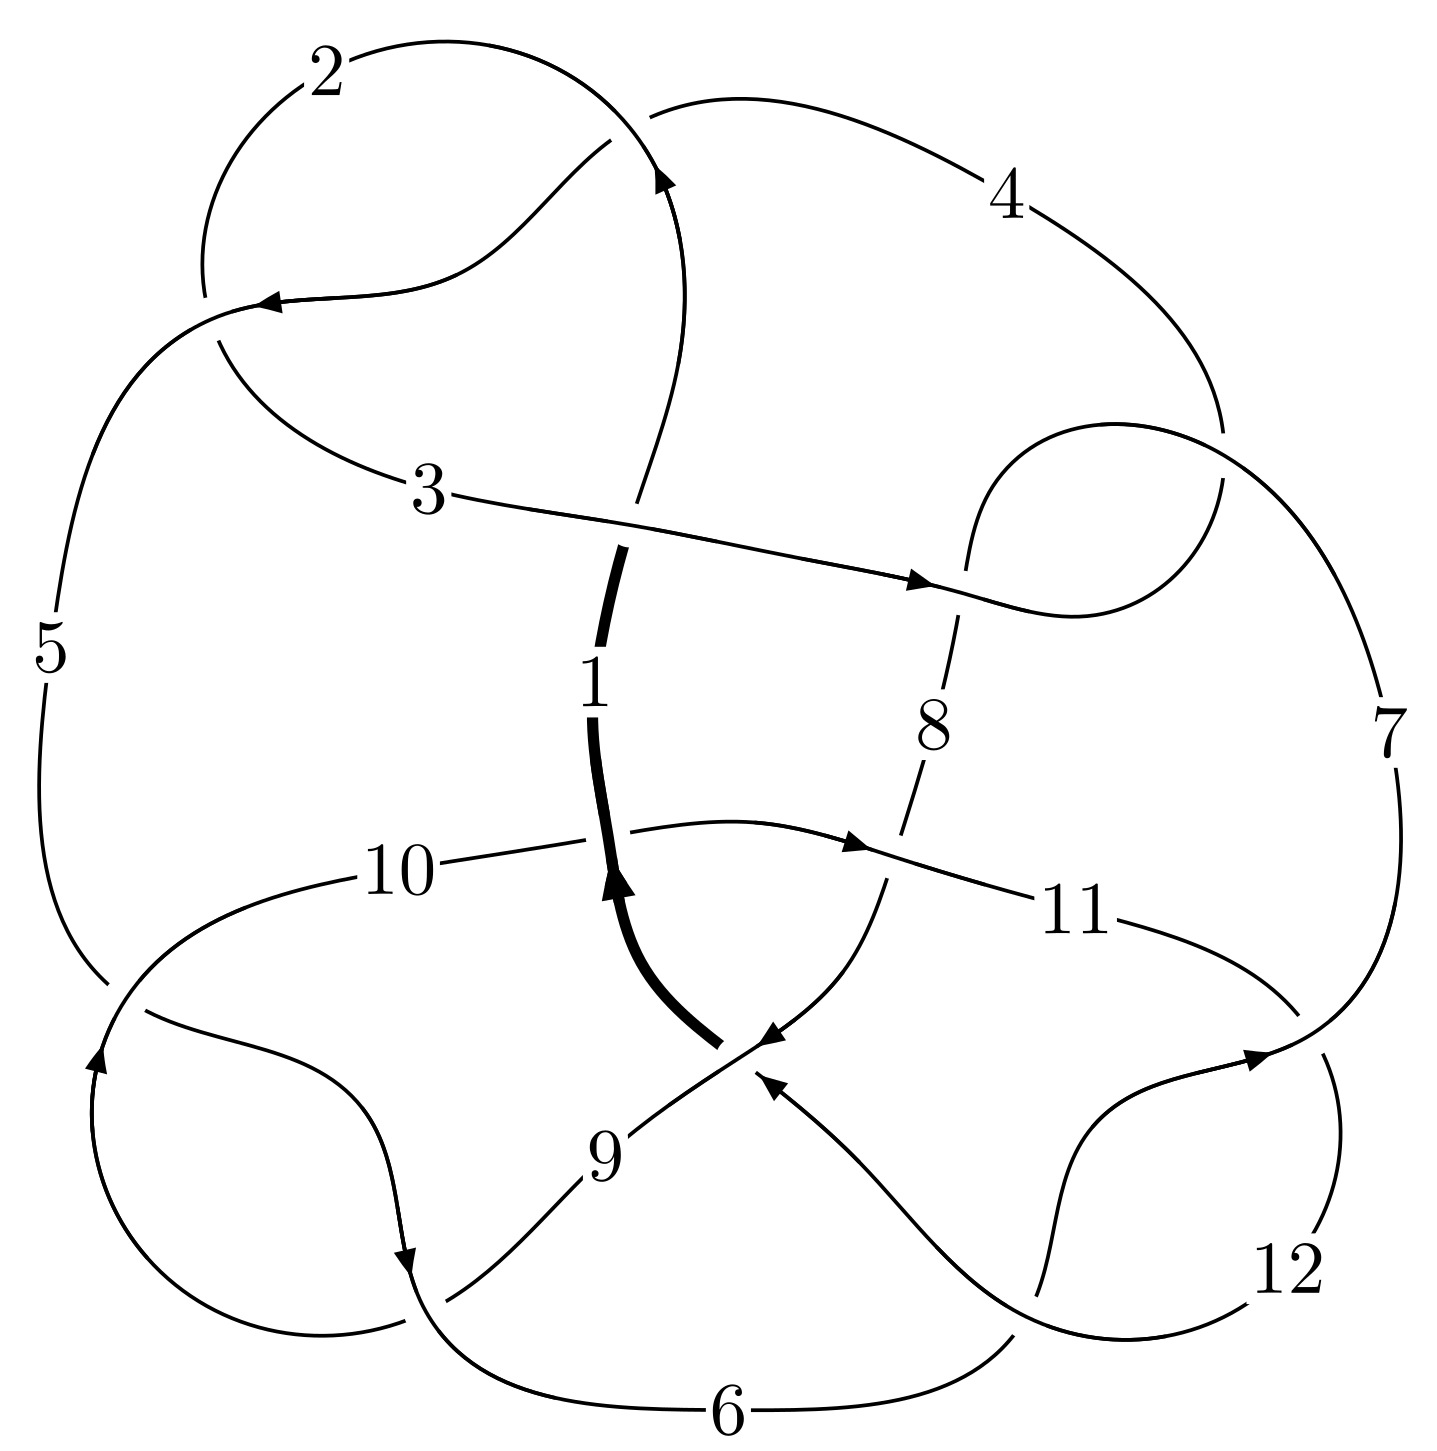
\includegraphics[width=112pt]{../../../GIT/diagram.site/Diagrams/png/2291_12n_0202.png}\\
\ \ \ A knot diagram\footnotemark}&
\allowdisplaybreaks
\textbf{Linearized knot diagam} \\
\cline{2-2}
 &
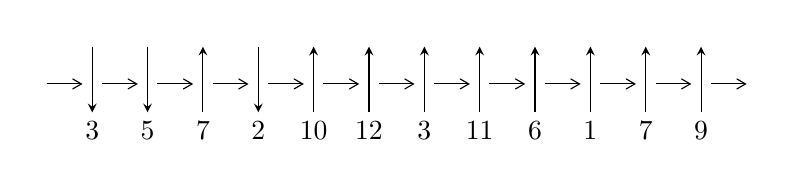
\begin{tikzpicture}[x=20pt, y=17pt]
	% nodes
	\node (C0) at (0, 0) {};
	\node (C1) at (1, 0) {};
	\node (C1U) at (1, +1) {};
	\node (C1D) at (1, -1) {3};

	\node (C2) at (2, 0) {};
	\node (C2U) at (2, +1) {};
	\node (C2D) at (2, -1) {5};

	\node (C3) at (3, 0) {};
	\node (C3U) at (3, +1) {};
	\node (C3D) at (3, -1) {7};

	\node (C4) at (4, 0) {};
	\node (C4U) at (4, +1) {};
	\node (C4D) at (4, -1) {2};

	\node (C5) at (5, 0) {};
	\node (C5U) at (5, +1) {};
	\node (C5D) at (5, -1) {10};

	\node (C6) at (6, 0) {};
	\node (C6U) at (6, +1) {};
	\node (C6D) at (6, -1) {12};

	\node (C7) at (7, 0) {};
	\node (C7U) at (7, +1) {};
	\node (C7D) at (7, -1) {3};

	\node (C8) at (8, 0) {};
	\node (C8U) at (8, +1) {};
	\node (C8D) at (8, -1) {11};

	\node (C9) at (9, 0) {};
	\node (C9U) at (9, +1) {};
	\node (C9D) at (9, -1) {6};

	\node (C10) at (10, 0) {};
	\node (C10U) at (10, +1) {};
	\node (C10D) at (10, -1) {1};

	\node (C11) at (11, 0) {};
	\node (C11U) at (11, +1) {};
	\node (C11D) at (11, -1) {7};

	\node (C12) at (12, 0) {};
	\node (C12U) at (12, +1) {};
	\node (C12D) at (12, -1) {9};
	\node (C13) at (13, 0) {};

	% arrows
	\draw[->,>={angle 60}]
	(C0) edge (C1) (C1) edge (C2) (C2) edge (C3) (C3) edge (C4) (C4) edge (C5) (C5) edge (C6) (C6) edge (C7) (C7) edge (C8) (C8) edge (C9) (C9) edge (C10) (C10) edge (C11) (C11) edge (C12) (C12) edge (C13) ;	\draw[->,>=stealth]
	(C1U) edge (C1D) (C2U) edge (C2D) (C3D) edge (C3U) (C4U) edge (C4D) (C5D) edge (C5U) (C6D) edge (C6U) (C7D) edge (C7U) (C8D) edge (C8U) (C9D) edge (C9U) (C10D) edge (C10U) (C11D) edge (C11U) (C12D) edge (C12U) ;
	\end{tikzpicture} \\
\hhline{~~} \\& 
\textbf{Solving Sequence} \\ \cline{2-2} 
 &
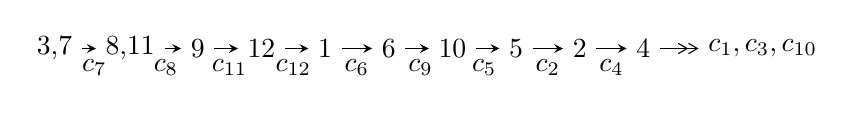
\begin{tikzpicture}[x=23pt, y=7pt]
	% node
	\node (A0) at (-1/8, 0) {3,7};
	\node (A1) at (17/16, 0) {8,11};
	\node (A2) at (17/8, 0) {9};
	\node (A3) at (25/8, 0) {12};
	\node (A4) at (33/8, 0) {1};
	\node (A5) at (41/8, 0) {6};
	\node (A6) at (49/8, 0) {10};
	\node (A7) at (57/8, 0) {5};
	\node (A8) at (65/8, 0) {2};
	\node (A9) at (73/8, 0) {4};
	\node (C1) at (1/2, -1) {$c_{7}$};
	\node (C2) at (13/8, -1) {$c_{8}$};
	\node (C3) at (21/8, -1) {$c_{11}$};
	\node (C4) at (29/8, -1) {$c_{12}$};
	\node (C5) at (37/8, -1) {$c_{6}$};
	\node (C6) at (45/8, -1) {$c_{9}$};
	\node (C7) at (53/8, -1) {$c_{5}$};
	\node (C8) at (61/8, -1) {$c_{2}$};
	\node (C9) at (69/8, -1) {$c_{4}$};
	\node (A10) at (11, 0) {$c_{1},c_{3},c_{10}$};

	% edge
	\draw[->,>=stealth]	
	(A0) edge (A1) (A1) edge (A2) (A2) edge (A3) (A3) edge (A4) (A4) edge (A5) (A5) edge (A6) (A6) edge (A7) (A7) edge (A8) (A8) edge (A9) ;
	\draw[->>,>={angle 60}]	
	(A9) edge (A10);
\end{tikzpicture} \\ 

\end{tabular} \\

\footnotetext{
The image of knot diagram is generated by the software ``\textbf{Draw programme}" developed by Andrew Bartholomew(\url{http://www.layer8.co.uk/maths/draw/index.htm\#Running-draw}), where we modified some parts for our purpose(\url{https://github.com/CATsTAILs/LinksPainter}).
}\phantom \\ \newline 
\centering \textbf{Ideals for irreducible components\footnotemark of $X_{\text{par}}$} 
 
\begin{align*}
I^u_{1}&=\langle 
2.05235\times10^{52} u^{33}+1.15512\times10^{53} u^{32}+\cdots+2.31768\times10^{52} b+6.87378\times10^{54},\\
\phantom{I^u_{1}}&\phantom{= \langle  }-8.21759\times10^{53} u^{33}-4.54814\times10^{54} u^{32}+\cdots+1.85414\times10^{53} a-2.27389\times10^{56},\\
\phantom{I^u_{1}}&\phantom{= \langle  }u^{34}+6 u^{33}+\cdots+1504 u+128\rangle \\
I^u_{2}&=\langle 
-185 u^{10} a^3+209 u^{10} a^2+\cdots-1226 a+794,\;6 u^{10} a^3+37 u^{10} a^2+\cdots-398 a-413,\\
\phantom{I^u_{2}}&\phantom{= \langle  }u^{11}+2 u^{10}- u^9-3 u^8+u^7+2 u^6+4 u^5+11 u^4+9 u^3+u^2-2 u-2\rangle \\
I^u_{3}&=\langle 
26139164 u^{15}+19494102 u^{14}+\cdots+39284803 b+1531021,\\
\phantom{I^u_{3}}&\phantom{= \langle  }221512445 u^{15}+269307859 u^{14}+\cdots+39284803 a+24902091,\\
\phantom{I^u_{3}}&\phantom{= \langle  }u^{16}+u^{15}- u^{14}-2 u^{13}-3 u^{12}-4 u^{11}+10 u^{10}+19 u^9+3 u^8-20 u^7-20 u^6+7 u^5+11 u^4+7 u^3+7 u^2+1\rangle \\
I^u_{4}&=\langle 
5698393 a^{11}+73535365 b+\cdots+1014170313 a-203703816,\\
\phantom{I^u_{4}}&\phantom{= \langle  }a^{12}-4 a^{11}+6 a^{10}-11 a^9+32 a^8-45 a^7+28 a^6-51 a^5+143 a^4-191 a^3+132 a^2-40 a+7,\;u-1\rangle \\
\\
I^v_{1}&=\langle 
a,\;-8 v^2+b+26 v-7,\;4 v^3-14 v^2+7 v-1\rangle \\
I^v_{2}&=\langle 
a,\;b^4- b^3+2 b^2-2 b+1,\;v+1\rangle \\
\end{align*}
\raggedright * 6 irreducible components of $\dim_{\mathbb{C}}=0$, with total 113 representations.\\
\footnotetext{All coefficients of polynomials are rational numbers. But the coefficients are sometimes approximated in decimal forms when there is not enough margin.}
\newpage
\renewcommand{\arraystretch}{1}
\centering \section*{I. $I^u_{1}= \langle 2.05\times10^{52} u^{33}+1.16\times10^{53} u^{32}+\cdots+2.32\times10^{52} b+6.87\times10^{54},\;-8.22\times10^{53} u^{33}-4.55\times10^{54} u^{32}+\cdots+1.85\times10^{53} a-2.27\times10^{56},\;u^{34}+6 u^{33}+\cdots+1504 u+128 \rangle$}
\flushleft \textbf{(i) Arc colorings}\\
\begin{tabular}{m{7pt} m{180pt} m{7pt} m{180pt} }
\flushright $a_{3}=$&$\begin{pmatrix}0\\u\end{pmatrix}$ \\
\flushright $a_{7}=$&$\begin{pmatrix}1\\0\end{pmatrix}$ \\
\flushright $a_{8}=$&$\begin{pmatrix}1\\- u^2\end{pmatrix}$ \\
\flushright $a_{11}=$&$\begin{pmatrix}4.43202 u^{33}+24.5296 u^{32}+\cdots+11740.1 u+1226.38\\-0.885519 u^{33}-4.98395 u^{32}+\cdots-2726.35 u-296.581\end{pmatrix}$ \\
\flushright $a_{9}=$&$\begin{pmatrix}3.82928 u^{33}+21.1964 u^{32}+\cdots+10122.3 u+1055.68\\1.77988 u^{33}+9.85723 u^{32}+\cdots+4665.13 u+481.509\end{pmatrix}$ \\
\flushright $a_{12}=$&$\begin{pmatrix}3.54650 u^{33}+19.5456 u^{32}+\cdots+9013.77 u+929.804\\-0.885519 u^{33}-4.98395 u^{32}+\cdots-2726.35 u-296.581\end{pmatrix}$ \\
\flushright $a_{1}=$&$\begin{pmatrix}1.06307 u^{33}+5.93274 u^{32}+\cdots+3043.91 u+325.793\\-2.44641 u^{33}-13.4720 u^{32}+\cdots-6083.54 u-619.031\end{pmatrix}$ \\
\flushright $a_{6}=$&$\begin{pmatrix}-0.691837 u^{33}-3.82621 u^{32}+\cdots-1770.73 u-179.020\\-2.07724 u^{33}-11.4986 u^{32}+\cdots-5450.40 u-563.433\end{pmatrix}$ \\
\flushright $a_{10}=$&$\begin{pmatrix}4.16237 u^{33}+23.1776 u^{32}+\cdots+11626.0 u+1231.40\\1.99898 u^{33}+11.2399 u^{32}+\cdots+6044.47 u+650.417\end{pmatrix}$ \\
\flushright $a_{5}=$&$\begin{pmatrix}3.32446 u^{33}+18.3671 u^{32}+\cdots+8593.18 u+887.775\\2.26139 u^{33}+12.4344 u^{32}+\cdots+5549.28 u+561.982\end{pmatrix}$ \\
\flushright $a_{2}=$&$\begin{pmatrix}1.06307 u^{33}+5.93274 u^{32}+\cdots+3043.91 u+325.793\\-2.26139 u^{33}-12.4344 u^{32}+\cdots-5549.28 u-561.982\end{pmatrix}$ \\
\flushright $a_{4}=$&$\begin{pmatrix}- u\\- u\end{pmatrix}$\\&\end{tabular}
\flushleft \textbf{(ii) Obstruction class $= -1$}\\~\\
\flushleft \textbf{(iii) Cusp Shapes $= -14.4745 u^{33}-80.2243 u^{32}+\cdots-38793.6 u-4044.27$}\\~\\
\newpage\renewcommand{\arraystretch}{1}
\flushleft \textbf{(iv) u-Polynomials at the component}\newline \\
\begin{tabular}{m{50pt}|m{274pt}}
Crossings & \hspace{64pt}u-Polynomials at each crossing \\
\hline $$\begin{aligned}c_{1}\end{aligned}$$&$\begin{aligned}
&u^{34}+19 u^{33}+\cdots+32880 u+256
\end{aligned}$\\
\hline $$\begin{aligned}c_{2},c_{4}\end{aligned}$$&$\begin{aligned}
&u^{34}-5 u^{33}+\cdots+204 u-16
\end{aligned}$\\
\hline $$\begin{aligned}c_{3},c_{7}\end{aligned}$$&$\begin{aligned}
&u^{34}-6 u^{33}+\cdots-1504 u+128
\end{aligned}$\\
\hline $$\begin{aligned}c_{5},c_{6},c_{9}\\c_{11}\end{aligned}$$&$\begin{aligned}
&u^{34}+12 u^{32}+\cdots- u-1
\end{aligned}$\\
\hline $$\begin{aligned}c_{8},c_{10}\end{aligned}$$&$\begin{aligned}
&u^{34}-8 u^{32}+\cdots+11 u+1
\end{aligned}$\\
\hline $$\begin{aligned}c_{12}\end{aligned}$$&$\begin{aligned}
&u^{34}-29 u^{33}+\cdots-229376 u+16384
\end{aligned}$\\
\hline
\end{tabular}\\~\\
\newpage\renewcommand{\arraystretch}{1}
\flushleft \textbf{(v) Riley Polynomials at the component}\newline \\
\begin{tabular}{m{50pt}|m{274pt}}
Crossings & \hspace{64pt}Riley Polynomials at each crossing \\
\hline $$\begin{aligned}c_{1}\end{aligned}$$&$\begin{aligned}
&y^{34}-3 y^{33}+\cdots-959098624 y+65536
\end{aligned}$\\
\hline $$\begin{aligned}c_{2},c_{4}\end{aligned}$$&$\begin{aligned}
&y^{34}-19 y^{33}+\cdots-32880 y+256
\end{aligned}$\\
\hline $$\begin{aligned}c_{3},c_{7}\end{aligned}$$&$\begin{aligned}
&y^{34}-12 y^{33}+\cdots-388096 y+16384
\end{aligned}$\\
\hline $$\begin{aligned}c_{5},c_{6},c_{9}\\c_{11}\end{aligned}$$&$\begin{aligned}
&y^{34}+24 y^{33}+\cdots- y+1
\end{aligned}$\\
\hline $$\begin{aligned}c_{8},c_{10}\end{aligned}$$&$\begin{aligned}
&y^{34}-16 y^{33}+\cdots-37 y+1
\end{aligned}$\\
\hline $$\begin{aligned}c_{12}\end{aligned}$$&$\begin{aligned}
&y^{34}+15 y^{33}+\cdots-536870912 y+268435456
\end{aligned}$\\
\hline
\end{tabular}\\~\\
\newpage\flushleft \textbf{(vi) Complex Volumes and Cusp Shapes}
$$\begin{array}{c|c|c}  
\text{Solutions to }I^u_{1}& \I (\text{vol} + \sqrt{-1}CS) & \text{Cusp shape}\\
 \hline 
\begin{aligned}
u &= -0.090643 + 0.777275 I \\
a &= \phantom{-}0.932410 + 0.812112 I \\
b &= -0.511224 + 0.237290 I\end{aligned}
 & \phantom{-}0.71635 + 1.25840 I & \phantom{-}9.52850 + 1.65312 I \\ \hline\begin{aligned}
u &= -0.090643 - 0.777275 I \\
a &= \phantom{-}0.932410 - 0.812112 I \\
b &= -0.511224 - 0.237290 I\end{aligned}
 & \phantom{-}0.71635 - 1.25840 I & \phantom{-}9.52850 - 1.65312 I \\ \hline\begin{aligned}
u &= \phantom{-}0.306658 + 0.718173 I \\
a &= \phantom{-}0.662294 - 0.462387 I \\
b &= \phantom{-}0.195615 - 0.391603 I\end{aligned}
 & -1.69600 - 0.85978 I & -1.64649 + 1.83237 I \\ \hline\begin{aligned}
u &= \phantom{-}0.306658 - 0.718173 I \\
a &= \phantom{-}0.662294 + 0.462387 I \\
b &= \phantom{-}0.195615 + 0.391603 I\end{aligned}
 & -1.69600 + 0.85978 I & -1.64649 - 1.83237 I \\ \hline\begin{aligned}
u &= \phantom{-}1.292730 + 0.093074 I \\
a &= -1.291070 + 0.061590 I \\
b &= \phantom{-}0.761362 - 0.484380 I\end{aligned}
 & \phantom{-}5.59278 + 0.13916 I & \phantom{-}9.58742 + 2.45732 I \\ \hline\begin{aligned}
u &= \phantom{-}1.292730 - 0.093074 I \\
a &= -1.291070 - 0.061590 I \\
b &= \phantom{-}0.761362 + 0.484380 I\end{aligned}
 & \phantom{-}5.59278 - 0.13916 I & \phantom{-}9.58742 - 2.45732 I \\ \hline\begin{aligned}
u &= -0.871052 + 0.990780 I \\
a &= -0.406604 - 0.666697 I \\
b &= -0.072976 - 0.925253 I\end{aligned}
 & -1.67974 + 1.56924 I & \phantom{-0.000000 } 0. - 1.70901 I \\ \hline\begin{aligned}
u &= -0.871052 - 0.990780 I \\
a &= -0.406604 + 0.666697 I \\
b &= -0.072976 + 0.925253 I\end{aligned}
 & -1.67974 - 1.56924 I & \phantom{-0.000000 -}0. + 1.70901 I \\ \hline\begin{aligned}
u &= -1.288240 + 0.420045 I \\
a &= -1.135880 - 0.354651 I \\
b &= \phantom{-}0.894899 + 0.322623 I\end{aligned}
 & \phantom{-}4.57328 - 5.79683 I & \phantom{-}6.00000 + 4.29308 I \\ \hline\begin{aligned}
u &= -1.288240 - 0.420045 I \\
a &= -1.135880 + 0.354651 I \\
b &= \phantom{-}0.894899 - 0.322623 I\end{aligned}
 & \phantom{-}4.57328 + 5.79683 I & \phantom{-}6.00000 - 4.29308 I\\
 \hline 
 \end{array}$$\newpage$$\begin{array}{c|c|c}  
\text{Solutions to }I^u_{1}& \I (\text{vol} + \sqrt{-1}CS) & \text{Cusp shape}\\
 \hline 
\begin{aligned}
u &= -1.304100 + 0.388118 I \\
a &= \phantom{-}1.251970 - 0.492836 I \\
b &= -0.510913 + 1.267090 I\end{aligned}
 & -6.83462 - 7.06965 I & \phantom{-0.000000 -}0. + 6.15439 I \\ \hline\begin{aligned}
u &= -1.304100 - 0.388118 I \\
a &= \phantom{-}1.251970 + 0.492836 I \\
b &= -0.510913 - 1.267090 I\end{aligned}
 & -6.83462 + 7.06965 I & \phantom{-0.000000 } 0. - 6.15439 I \\ \hline\begin{aligned}
u &= -1.359360 + 0.205447 I \\
a &= \phantom{-}0.692011 + 0.175208 I \\
b &= -0.778312 - 0.579500 I\end{aligned}
 & \phantom{-}3.00226 - 0.76687 I & \phantom{-}6.00000 + 0. I\phantom{ +0.000000I} \\ \hline\begin{aligned}
u &= -1.359360 - 0.205447 I \\
a &= \phantom{-}0.692011 - 0.175208 I \\
b &= -0.778312 + 0.579500 I\end{aligned}
 & \phantom{-}3.00226 + 0.76687 I & \phantom{-}6.00000 + 0. I\phantom{ +0.000000I} \\ \hline\begin{aligned}
u &= \phantom{-}1.154680 + 0.767394 I \\
a &= -0.894645 + 0.517297 I \\
b &= \phantom{-}0.262146 + 0.969895 I\end{aligned}
 & \phantom{-}2.68203 + 3.10270 I & \phantom{-}6.00000 + 0. I\phantom{ +0.000000I} \\ \hline\begin{aligned}
u &= \phantom{-}1.154680 - 0.767394 I \\
a &= -0.894645 - 0.517297 I \\
b &= \phantom{-}0.262146 - 0.969895 I\end{aligned}
 & \phantom{-}2.68203 - 3.10270 I & \phantom{-}6.00000 + 0. I\phantom{ +0.000000I} \\ \hline\begin{aligned}
u &= -0.510540 + 1.313970 I \\
a &= -0.051694 + 0.350554 I \\
b &= \phantom{-}0.55842 + 1.32975 I\end{aligned}
 & -5.67028 + 10.25340 I & \phantom{-0.000000 } 0. - 7.14529 I \\ \hline\begin{aligned}
u &= -0.510540 - 1.313970 I \\
a &= -0.051694 - 0.350554 I \\
b &= \phantom{-}0.55842 - 1.32975 I\end{aligned}
 & -5.67028 - 10.25340 I & \phantom{-0.000000 -}0. + 7.14529 I \\ \hline\begin{aligned}
u &= \phantom{-}0.286604 + 1.384360 I \\
a &= -0.024163 - 0.361453 I \\
b &= \phantom{-}0.503949 - 1.158680 I\end{aligned}
 & -4.18172 - 4.31448 I & \phantom{-0.000000 } 0 \\ \hline\begin{aligned}
u &= \phantom{-}0.286604 - 1.384360 I \\
a &= -0.024163 + 0.361453 I \\
b &= \phantom{-}0.503949 + 1.158680 I\end{aligned}
 & -4.18172 + 4.31448 I & \phantom{-0.000000 } 0\\
 \hline 
 \end{array}$$\newpage$$\begin{array}{c|c|c}  
\text{Solutions to }I^u_{1}& \I (\text{vol} + \sqrt{-1}CS) & \text{Cusp shape}\\
 \hline 
\begin{aligned}
u &= -1.20850 + 0.89083 I \\
a &= -0.923171 - 0.397480 I \\
b &= \phantom{-}0.237804 - 1.150510 I\end{aligned}
 & -0.57232 - 8.89823 I & \phantom{-0.000000 } 0 \\ \hline\begin{aligned}
u &= -1.20850 - 0.89083 I \\
a &= -0.923171 + 0.397480 I \\
b &= \phantom{-}0.237804 + 1.150510 I\end{aligned}
 & -0.57232 + 8.89823 I & \phantom{-0.000000 } 0 \\ \hline\begin{aligned}
u &= \phantom{-}1.52570 + 0.09137 I \\
a &= \phantom{-}0.736791 + 0.196904 I \\
b &= -0.716836 - 0.876660 I\end{aligned}
 & \phantom{-}3.16512 + 5.42087 I & \phantom{-0.000000 } 0 \\ \hline\begin{aligned}
u &= \phantom{-}1.52570 - 0.09137 I \\
a &= \phantom{-}0.736791 - 0.196904 I \\
b &= -0.716836 + 0.876660 I\end{aligned}
 & \phantom{-}3.16512 - 5.42087 I & \phantom{-0.000000 } 0 \\ \hline\begin{aligned}
u &= -0.463998\phantom{ +0.000000I} \\
a &= -5.35214\phantom{ +0.000000I} \\
b &= \phantom{-}0.401353\phantom{ +0.000000I}\end{aligned}
 & -0.541158\phantom{ +0.000000I} & \phantom{-}31.3900\phantom{ +0.000000I} \\ \hline\begin{aligned}
u &= -1.32019 + 0.79594 I \\
a &= \phantom{-}1.40106 + 0.21908 I \\
b &= -0.61404 + 1.47259 I\end{aligned}
 & -2.9964 - 17.7107 I & \phantom{-0.000000 } 0 \\ \hline\begin{aligned}
u &= -1.32019 - 0.79594 I \\
a &= \phantom{-}1.40106 - 0.21908 I \\
b &= -0.61404 - 1.47259 I\end{aligned}
 & -2.9964 + 17.7107 I & \phantom{-0.000000 } 0 \\ \hline\begin{aligned}
u &= -0.448045 + 0.057573 I \\
a &= -0.050536 + 0.333276 I \\
b &= \phantom{-}0.22589 + 1.49925 I\end{aligned}
 & -10.84120 + 5.04921 I & \phantom{-}15.4774 + 2.0506 I \\ \hline\begin{aligned}
u &= -0.448045 - 0.057573 I \\
a &= -0.050536 - 0.333276 I \\
b &= \phantom{-}0.22589 - 1.49925 I\end{aligned}
 & -10.84120 - 5.04921 I & \phantom{-}15.4774 - 2.0506 I \\ \hline\begin{aligned}
u &= \phantom{-}1.40945 + 0.64929 I \\
a &= \phantom{-}1.283140 - 0.005753 I \\
b &= -0.63967 - 1.38569 I\end{aligned}
 & -0.33266 + 11.43620 I & \phantom{-0.000000 } 0\\
 \hline 
 \end{array}$$\newpage$$\begin{array}{c|c|c}  
\text{Solutions to }I^u_{1}& \I (\text{vol} + \sqrt{-1}CS) & \text{Cusp shape}\\
 \hline 
\begin{aligned}
u &= \phantom{-}1.40945 - 0.64929 I \\
a &= \phantom{-}1.283140 + 0.005753 I \\
b &= -0.63967 + 1.38569 I\end{aligned}
 & -0.33266 - 11.43620 I & \phantom{-0.000000 } 0 \\ \hline\begin{aligned}
u &= -0.19301 + 1.65922 I \\
a &= \phantom{-}0.049963 + 0.259298 I \\
b &= \phantom{-}0.220997 + 0.996367 I\end{aligned}
 & -12.14010 + 0.90472 I & \phantom{-0.000000 } 0 \\ \hline\begin{aligned}
u &= -0.19301 - 1.65922 I \\
a &= \phantom{-}0.049963 - 0.259298 I \\
b &= \phantom{-}0.220997 - 0.996367 I\end{aligned}
 & -12.14010 - 0.90472 I & \phantom{-0.000000 } 0 \\ \hline\begin{aligned}
u &= -0.300279\phantom{ +0.000000I} \\
a &= \phantom{-}1.01338\phantom{ +0.000000I} \\
b &= -0.435581\phantom{ +0.000000I}\end{aligned}
 & \phantom{-}0.684542\phantom{ +0.000000I} & \phantom{-}14.6620\phantom{ +0.000000I}\\
 \hline 
 \end{array}$$\newpage\newpage\renewcommand{\arraystretch}{1}
\centering \section*{II. $I^u_{2}= \langle -185 u^{10} a^3+209 u^{10} a^2+\cdots-1226 a+794,\;6 u^{10} a^3+37 u^{10} a^2+\cdots-398 a-413,\;u^{11}+2 u^{10}+\cdots-2 u-2 \rangle$}
\flushleft \textbf{(i) Arc colorings}\\
\begin{tabular}{m{7pt} m{180pt} m{7pt} m{180pt} }
\flushright $a_{3}=$&$\begin{pmatrix}0\\u\end{pmatrix}$ \\
\flushright $a_{7}=$&$\begin{pmatrix}1\\0\end{pmatrix}$ \\
\flushright $a_{8}=$&$\begin{pmatrix}1\\- u^2\end{pmatrix}$ \\
\flushright $a_{11}=$&$\begin{pmatrix}a\\0.690299 a^{3} u^{10}-0.779851 a^{2} u^{10}+\cdots+4.57463 a-2.96269\end{pmatrix}$ \\
\flushright $a_{9}=$&$\begin{pmatrix}-0.470149 a^{3} u^{10}+0.279851 a^{2} u^{10}+\cdots-3.03731 a+0.462687\\0.0298507 a^{2} u^{10}+0.485075 u^{10}+\cdots+0.0746269 a^{2}+0.462687\end{pmatrix}$ \\
\flushright $a_{12}=$&$\begin{pmatrix}0.690299 a^{3} u^{10}-0.779851 a^{2} u^{10}+\cdots+5.57463 a-2.96269\\0.690299 a^{3} u^{10}-0.779851 a^{2} u^{10}+\cdots+4.57463 a-2.96269\end{pmatrix}$ \\
\flushright $a_{1}=$&$\begin{pmatrix}\frac{1}{2} u^{10}+\frac{3}{4} u^9+\cdots+\frac{11}{4} u^2-\frac{3}{2}\\\frac{1}{2} u^{10}+\frac{1}{2} u^9+\cdots+\frac{7}{4} u^2-\frac{1}{2}\end{pmatrix}$ \\
\flushright $a_{6}=$&$\begin{pmatrix}-0.100746 a^{3} u^{10}-0.380597 a^{2} u^{10}+\cdots+0.313433 a+0.850746\\-0.570896 a^{3} u^{10}-0.100746 a^{2} u^{10}+\cdots-2.72388 a-0.686567\end{pmatrix}$ \\
\flushright $a_{10}=$&$\begin{pmatrix}0.0597015 a^{3} u^{10}-0.220149 a^{2} u^{10}+\cdots+1.42537 a-3.03731\\0.559701 a^{3} u^{10}-0.970149 a^{2} u^{10}+\cdots+5.42537 a-4.03731\end{pmatrix}$ \\
\flushright $a_{5}=$&$\begin{pmatrix}-\frac{1}{4} u^{10}+\frac{3}{4} u^8+\cdots-\frac{1}{2} u-\frac{1}{2}\\-\frac{3}{4} u^{10}-\frac{3}{4} u^9+\cdots-\frac{1}{2} u+1\end{pmatrix}$ \\
\flushright $a_{2}=$&$\begin{pmatrix}\frac{1}{2} u^{10}+\frac{3}{4} u^9+\cdots+\frac{11}{4} u^2-\frac{3}{2}\\\frac{3}{4} u^{10}+\frac{3}{4} u^9+\cdots+\frac{1}{2} u-1\end{pmatrix}$ \\
\flushright $a_{4}=$&$\begin{pmatrix}- u\\- u\end{pmatrix}$\\&\end{tabular}
\flushleft \textbf{(ii) Obstruction class $= -1$}\\~\\
\flushleft \textbf{(iii) Cusp Shapes $= \frac{83}{67} u^{10} a^3-\frac{126}{67} u^{10} a^2+\cdots+\frac{784}{67} a-\frac{144}{67}$}\\~\\
\newpage\renewcommand{\arraystretch}{1}
\flushleft \textbf{(iv) u-Polynomials at the component}\newline \\
\begin{tabular}{m{50pt}|m{274pt}}
Crossings & \hspace{64pt}u-Polynomials at each crossing \\
\hline $$\begin{aligned}c_{1}\end{aligned}$$&$\begin{aligned}
&(u^{11}+4 u^{10}+\cdots+11 u+1)^{4}
\end{aligned}$\\
\hline $$\begin{aligned}c_{2},c_{4}\end{aligned}$$&$\begin{aligned}
&(u^{11}-2 u^{10}+4 u^8-2 u^7-4 u^6+5 u^5+2 u^4-5 u^3+u^2+3 u-1)^4
\end{aligned}$\\
\hline $$\begin{aligned}c_{3},c_{7}\end{aligned}$$&$\begin{aligned}
&(u^{11}-2 u^{10}- u^9+3 u^8+u^7-2 u^6+4 u^5-11 u^4+9 u^3- u^2-2 u+2)^4
\end{aligned}$\\
\hline $$\begin{aligned}c_{5},c_{6},c_{9}\\c_{11}\end{aligned}$$&$\begin{aligned}
&u^{44}-2 u^{43}+\cdots+2932 u+661
\end{aligned}$\\
\hline $$\begin{aligned}c_{8},c_{10}\end{aligned}$$&$\begin{aligned}
&u^{44}+10 u^{43}+\cdots+1758 u+421
\end{aligned}$\\
\hline $$\begin{aligned}c_{12}\end{aligned}$$&$\begin{aligned}
&(u^2+u+1)^{22}
\end{aligned}$\\
\hline
\end{tabular}\\~\\
\newpage\renewcommand{\arraystretch}{1}
\flushleft \textbf{(v) Riley Polynomials at the component}\newline \\
\begin{tabular}{m{50pt}|m{274pt}}
Crossings & \hspace{64pt}Riley Polynomials at each crossing \\
\hline $$\begin{aligned}c_{1}\end{aligned}$$&$\begin{aligned}
&(y^{11}+8 y^{10}+\cdots+67 y-1)^{4}
\end{aligned}$\\
\hline $$\begin{aligned}c_{2},c_{4}\end{aligned}$$&$\begin{aligned}
&(y^{11}-4 y^{10}+\cdots+11 y-1)^{4}
\end{aligned}$\\
\hline $$\begin{aligned}c_{3},c_{7}\end{aligned}$$&$\begin{aligned}
&(y^{11}-6 y^{10}+\cdots+8 y-4)^{4}
\end{aligned}$\\
\hline $$\begin{aligned}c_{5},c_{6},c_{9}\\c_{11}\end{aligned}$$&$\begin{aligned}
&y^{44}+30 y^{43}+\cdots+6318180 y+436921
\end{aligned}$\\
\hline $$\begin{aligned}c_{8},c_{10}\end{aligned}$$&$\begin{aligned}
&y^{44}-2 y^{43}+\cdots-1105128 y+177241
\end{aligned}$\\
\hline $$\begin{aligned}c_{12}\end{aligned}$$&$\begin{aligned}
&(y^2+y+1)^{22}
\end{aligned}$\\
\hline
\end{tabular}\\~\\
\newpage\flushleft \textbf{(vi) Complex Volumes and Cusp Shapes}
$$\begin{array}{c|c|c}  
\text{Solutions to }I^u_{2}& \I (\text{vol} + \sqrt{-1}CS) & \text{Cusp shape}\\
 \hline 
\begin{aligned}
u &= \phantom{-}0.217339 + 1.116860 I \\
a &= -0.009955 + 0.594446 I \\
b &= \phantom{-}1.080720 + 0.060619 I\end{aligned}
 & -1.72919 - 4.44881 I & \phantom{-}2.92816 + 6.35357 I \\ \hline\begin{aligned}
u &= \phantom{-}0.217339 + 1.116860 I \\
a &= \phantom{-}0.443379 + 0.335985 I \\
b &= -0.301589 + 1.082120 I\end{aligned}
 & -1.72919 - 4.44881 I & \phantom{-}2.92816 + 6.35357 I \\ \hline\begin{aligned}
u &= \phantom{-}0.217339 + 1.116860 I \\
a &= \phantom{-}0.183122 - 0.512572 I \\
b &= \phantom{-}0.700289 - 0.364504 I\end{aligned}
 & -1.72919 - 0.38904 I & \phantom{-}2.92816 - 0.57463 I \\ \hline\begin{aligned}
u &= \phantom{-}0.217339 + 1.116860 I \\
a &= \phantom{-}0.405942 - 0.327999 I \\
b &= -0.100215 - 0.881617 I\end{aligned}
 & -1.72919 - 0.38904 I & \phantom{-}2.92816 - 0.57463 I \\ \hline\begin{aligned}
u &= \phantom{-}0.217339 - 1.116860 I \\
a &= -0.009955 - 0.594446 I \\
b &= \phantom{-}1.080720 - 0.060619 I\end{aligned}
 & -1.72919 + 4.44881 I & \phantom{-}2.92816 - 6.35357 I \\ \hline\begin{aligned}
u &= \phantom{-}0.217339 - 1.116860 I \\
a &= \phantom{-}0.443379 - 0.335985 I \\
b &= -0.301589 - 1.082120 I\end{aligned}
 & -1.72919 + 4.44881 I & \phantom{-}2.92816 - 6.35357 I \\ \hline\begin{aligned}
u &= \phantom{-}0.217339 - 1.116860 I \\
a &= \phantom{-}0.183122 + 0.512572 I \\
b &= \phantom{-}0.700289 + 0.364504 I\end{aligned}
 & -1.72919 + 0.38904 I & \phantom{-}2.92816 + 0.57463 I \\ \hline\begin{aligned}
u &= \phantom{-}0.217339 - 1.116860 I \\
a &= \phantom{-}0.405942 + 0.327999 I \\
b &= -0.100215 + 0.881617 I\end{aligned}
 & -1.72919 + 0.38904 I & \phantom{-}2.92816 + 0.57463 I \\ \hline\begin{aligned}
u &= -1.116820 + 0.404951 I \\
a &= \phantom{-}0.367564 + 1.052860 I \\
b &= -0.088366 + 1.407570 I\end{aligned}
 & -4.26357 - 6.72730 I & \phantom{-}0.91876 + 9.34733 I \\ \hline\begin{aligned}
u &= -1.116820 + 0.404951 I \\
a &= -1.61003 + 0.21622 I \\
b &= \phantom{-}0.97212 - 1.45656 I\end{aligned}
 & -4.26357 - 6.72730 I & \phantom{-}0.91876 + 9.34733 I\\
 \hline 
 \end{array}$$\newpage$$\begin{array}{c|c|c}  
\text{Solutions to }I^u_{2}& \I (\text{vol} + \sqrt{-1}CS) & \text{Cusp shape}\\
 \hline 
\begin{aligned}
u &= -1.116820 + 0.404951 I \\
a &= -0.153427 + 0.275989 I \\
b &= -0.38639 - 1.80698 I\end{aligned}
 & -4.26357 - 2.66753 I & \phantom{-}0.91876 + 2.41912 I \\ \hline\begin{aligned}
u &= -1.116820 + 0.404951 I \\
a &= \phantom{-}1.87372 + 0.16548 I \\
b &= -0.097911 + 1.066130 I\end{aligned}
 & -4.26357 - 2.66753 I & \phantom{-}0.91876 + 2.41912 I \\ \hline\begin{aligned}
u &= -1.116820 - 0.404951 I \\
a &= \phantom{-}0.367564 - 1.052860 I \\
b &= -0.088366 - 1.407570 I\end{aligned}
 & -4.26357 + 6.72730 I & \phantom{-}0.91876 - 9.34733 I \\ \hline\begin{aligned}
u &= -1.116820 - 0.404951 I \\
a &= -1.61003 - 0.21622 I \\
b &= \phantom{-}0.97212 + 1.45656 I\end{aligned}
 & -4.26357 + 6.72730 I & \phantom{-}0.91876 - 9.34733 I \\ \hline\begin{aligned}
u &= -1.116820 - 0.404951 I \\
a &= -0.153427 - 0.275989 I \\
b &= -0.38639 + 1.80698 I\end{aligned}
 & -4.26357 + 2.66753 I & \phantom{-}0.91876 - 2.41912 I \\ \hline\begin{aligned}
u &= -1.116820 - 0.404951 I \\
a &= \phantom{-}1.87372 - 0.16548 I \\
b &= -0.097911 - 1.066130 I\end{aligned}
 & -4.26357 + 2.66753 I & \phantom{-}0.91876 - 2.41912 I \\ \hline\begin{aligned}
u &= -0.323694 + 0.583510 I \\
a &= -2.18729 + 0.34333 I \\
b &= -0.58191 - 1.32255 I\end{aligned}
 & -6.66575 + 2.77184 I & -5.53927 - 4.58319 I \\ \hline\begin{aligned}
u &= -0.323694 + 0.583510 I \\
a &= -0.81002 + 2.90630 I \\
b &= -0.184279 + 1.140270 I\end{aligned}
 & -6.66575 - 1.28793 I & -5.53927 + 2.34501 I \\ \hline\begin{aligned}
u &= -0.323694 + 0.583510 I \\
a &= -4.27663 - 3.61387 I \\
b &= \phantom{-}0.41189 - 1.47115 I\end{aligned}
 & -6.66575 - 1.28793 I & -5.53927 + 2.34501 I \\ \hline\begin{aligned}
u &= -0.323694 + 0.583510 I \\
a &= \phantom{-}4.11785 + 4.41562 I \\
b &= \phantom{-}0.181553 + 1.290880 I\end{aligned}
 & -6.66575 + 2.77184 I & -5.53927 - 4.58319 I\\
 \hline 
 \end{array}$$\newpage$$\begin{array}{c|c|c}  
\text{Solutions to }I^u_{2}& \I (\text{vol} + \sqrt{-1}CS) & \text{Cusp shape}\\
 \hline 
\begin{aligned}
u &= -0.323694 - 0.583510 I \\
a &= -2.18729 - 0.34333 I \\
b &= -0.58191 + 1.32255 I\end{aligned}
 & -6.66575 - 2.77184 I & -5.53927 + 4.58319 I \\ \hline\begin{aligned}
u &= -0.323694 - 0.583510 I \\
a &= -0.81002 - 2.90630 I \\
b &= -0.184279 - 1.140270 I\end{aligned}
 & -6.66575 + 1.28793 I & -5.53927 - 2.34501 I \\ \hline\begin{aligned}
u &= -0.323694 - 0.583510 I \\
a &= -4.27663 + 3.61387 I \\
b &= \phantom{-}0.41189 + 1.47115 I\end{aligned}
 & -6.66575 + 1.28793 I & -5.53927 - 2.34501 I \\ \hline\begin{aligned}
u &= -0.323694 - 0.583510 I \\
a &= \phantom{-}4.11785 - 4.41562 I \\
b &= \phantom{-}0.181553 - 1.290880 I\end{aligned}
 & -6.66575 - 2.77184 I & -5.53927 + 4.58319 I \\ \hline\begin{aligned}
u &= -1.38823 + 0.36743 I \\
a &= \phantom{-}1.002740 + 0.157516 I \\
b &= -0.899581 + 0.768683 I\end{aligned}
 & \phantom{-}3.68097 - 0.55463 I & \phantom{-}6.19194 - 2.44750 I \\ \hline\begin{aligned}
u &= -1.38823 + 0.36743 I \\
a &= \phantom{-}1.150210 + 0.262394 I \\
b &= -1.349990 - 0.139533 I\end{aligned}
 & \phantom{-}3.68097 - 4.61439 I & \phantom{-}6.19194 + 4.48070 I \\ \hline\begin{aligned}
u &= -1.38823 + 0.36743 I \\
a &= -1.318500 + 0.350190 I \\
b &= \phantom{-}0.442958 - 1.080190 I\end{aligned}
 & \phantom{-}3.68097 - 4.61439 I & \phantom{-}6.19194 + 4.48070 I \\ \hline\begin{aligned}
u &= -1.38823 + 0.36743 I \\
a &= -0.388078 - 0.318066 I \\
b &= \phantom{-}0.296789 + 0.626688 I\end{aligned}
 & \phantom{-}3.68097 - 0.55463 I & \phantom{-}6.19194 - 2.44750 I \\ \hline\begin{aligned}
u &= -1.38823 - 0.36743 I \\
a &= \phantom{-}1.002740 - 0.157516 I \\
b &= -0.899581 - 0.768683 I\end{aligned}
 & \phantom{-}3.68097 + 0.55463 I & \phantom{-}6.19194 + 2.44750 I \\ \hline\begin{aligned}
u &= -1.38823 - 0.36743 I \\
a &= \phantom{-}1.150210 - 0.262394 I \\
b &= -1.349990 + 0.139533 I\end{aligned}
 & \phantom{-}3.68097 + 4.61439 I & \phantom{-}6.19194 - 4.48070 I\\
 \hline 
 \end{array}$$\newpage$$\begin{array}{c|c|c}  
\text{Solutions to }I^u_{2}& \I (\text{vol} + \sqrt{-1}CS) & \text{Cusp shape}\\
 \hline 
\begin{aligned}
u &= -1.38823 - 0.36743 I \\
a &= -1.318500 - 0.350190 I \\
b &= \phantom{-}0.442958 + 1.080190 I\end{aligned}
 & \phantom{-}3.68097 + 4.61439 I & \phantom{-}6.19194 - 4.48070 I \\ \hline\begin{aligned}
u &= -1.38823 - 0.36743 I \\
a &= -0.388078 + 0.318066 I \\
b &= \phantom{-}0.296789 - 0.626688 I\end{aligned}
 & \phantom{-}3.68097 + 0.55463 I & \phantom{-}6.19194 + 2.44750 I \\ \hline\begin{aligned}
u &= \phantom{-}0.552641\phantom{ +0.000000I} \\
a &= \phantom{-}0.753677 + 0.114672 I \\
b &= -0.156468 + 1.382340 I\end{aligned}
 & -3.80862 - 2.02988 I & \phantom{-}7.42944 + 3.46410 I \\ \hline\begin{aligned}
u &= \phantom{-}0.552641\phantom{ +0.000000I} \\
a &= \phantom{-}0.753677 - 0.114672 I \\
b &= -0.156468 - 1.382340 I\end{aligned}
 & -3.80862 + 2.02988 I & \phantom{-}7.42944 - 3.46410 I \\ \hline\begin{aligned}
u &= \phantom{-}0.552641\phantom{ +0.000000I} \\
a &= \phantom{-}0.24741 + 1.61926 I \\
b &= \phantom{-}0.546490 - 0.706801 I\end{aligned}
 & -3.80862 - 2.02988 I & \phantom{-}7.42944 + 3.46410 I \\ \hline\begin{aligned}
u &= \phantom{-}0.552641\phantom{ +0.000000I} \\
a &= \phantom{-}0.24741 - 1.61926 I \\
b &= \phantom{-}0.546490 + 0.706801 I\end{aligned}
 & -3.80862 + 2.02988 I & \phantom{-}7.42944 - 3.46410 I \\ \hline\begin{aligned}
u &= \phantom{-}1.33508 + 0.61220 I \\
a &= \phantom{-}1.056630 - 0.199046 I \\
b &= -0.774609 - 1.057170 I\end{aligned}
 & \phantom{-}1.83471 + 6.62127 I & \phantom{-}3.78570 - 2.11482 I \\ \hline\begin{aligned}
u &= \phantom{-}1.33508 + 0.61220 I \\
a &= \phantom{-}1.069070 - 0.482704 I \\
b &= -1.45883 - 0.04222 I\end{aligned}
 & \phantom{-}1.83471 + 10.68100 I & \phantom{-}3.78570 - 9.04302 I \\ \hline\begin{aligned}
u &= \phantom{-}1.33508 + 0.61220 I \\
a &= -1.53253 - 0.02543 I \\
b &= \phantom{-}0.460172 + 1.181660 I\end{aligned}
 & \phantom{-}1.83471 + 10.68100 I & \phantom{-}3.78570 - 9.04302 I \\ \hline\begin{aligned}
u &= \phantom{-}1.33508 + 0.61220 I \\
a &= -0.384837 + 0.051738 I \\
b &= \phantom{-}0.287156 - 0.377419 I\end{aligned}
 & \phantom{-}1.83471 + 6.62127 I & \phantom{-}3.78570 - 2.11482 I\\
 \hline 
 \end{array}$$\newpage$$\begin{array}{c|c|c}  
\text{Solutions to }I^u_{2}& \I (\text{vol} + \sqrt{-1}CS) & \text{Cusp shape}\\
 \hline 
\begin{aligned}
u &= \phantom{-}1.33508 - 0.61220 I \\
a &= \phantom{-}1.056630 + 0.199046 I \\
b &= -0.774609 + 1.057170 I\end{aligned}
 & \phantom{-}1.83471 - 6.62127 I & \phantom{-}3.78570 + 2.11482 I \\ \hline\begin{aligned}
u &= \phantom{-}1.33508 - 0.61220 I \\
a &= \phantom{-}1.069070 + 0.482704 I \\
b &= -1.45883 + 0.04222 I\end{aligned}
 & \phantom{-}1.83471 - 10.68100 I & \phantom{-}3.78570 + 9.04302 I \\ \hline\begin{aligned}
u &= \phantom{-}1.33508 - 0.61220 I \\
a &= -1.53253 + 0.02543 I \\
b &= \phantom{-}0.460172 - 1.181660 I\end{aligned}
 & \phantom{-}1.83471 - 10.68100 I & \phantom{-}3.78570 + 9.04302 I \\ \hline\begin{aligned}
u &= \phantom{-}1.33508 - 0.61220 I \\
a &= -0.384837 - 0.051738 I \\
b &= \phantom{-}0.287156 + 0.377419 I\end{aligned}
 & \phantom{-}1.83471 - 6.62127 I & \phantom{-}3.78570 + 2.11482 I\\
 \hline 
 \end{array}$$\newpage\newpage\renewcommand{\arraystretch}{1}
\centering \section*{III. $I^u_{3}= \langle 2.61\times10^{7} u^{15}+1.95\times10^{7} u^{14}+\cdots+3.93\times10^{7} b+1.53\times10^{6},\;2.22\times10^{8} u^{15}+2.69\times10^{8} u^{14}+\cdots+3.93\times10^{7} a+2.49\times10^{7},\;u^{16}+u^{15}+\cdots+7 u^2+1 \rangle$}
\flushleft \textbf{(i) Arc colorings}\\
\begin{tabular}{m{7pt} m{180pt} m{7pt} m{180pt} }
\flushright $a_{3}=$&$\begin{pmatrix}0\\u\end{pmatrix}$ \\
\flushright $a_{7}=$&$\begin{pmatrix}1\\0\end{pmatrix}$ \\
\flushright $a_{8}=$&$\begin{pmatrix}1\\- u^2\end{pmatrix}$ \\
\flushright $a_{11}=$&$\begin{pmatrix}-5.63863 u^{15}-6.85527 u^{14}+\cdots-37.3060 u-0.633886\\-0.665376 u^{15}-0.496225 u^{14}+\cdots-3.75673 u-0.0389723\end{pmatrix}$ \\
\flushright $a_{9}=$&$\begin{pmatrix}4.79895 u^{15}+4.13796 u^{14}+\cdots+13.0962 u-10.2774\\0.824960 u^{15}+0.614372 u^{14}+\cdots+2.39162 u-0.704160\end{pmatrix}$ \\
\flushright $a_{12}=$&$\begin{pmatrix}-6.30401 u^{15}-7.35149 u^{14}+\cdots-41.0628 u-0.672858\\-0.665376 u^{15}-0.496225 u^{14}+\cdots-3.75673 u-0.0389723\end{pmatrix}$ \\
\flushright $a_{1}=$&$\begin{pmatrix}-0.839243 u^{15}-0.933409 u^{14}+\cdots-5.49869 u-0.251285\\-0.0768567 u^{15}-0.0612071 u^{14}+\cdots-0.173867 u-0.263317\end{pmatrix}$ \\
\flushright $a_{6}=$&$\begin{pmatrix}0.471243 u^{15}-2.73305 u^{14}+\cdots-23.9979 u-20.9855\\-0.0384779 u^{15}-0.360948 u^{14}+\cdots-1.88190 u-2.17767\end{pmatrix}$ \\
\flushright $a_{10}=$&$\begin{pmatrix}-6.46359 u^{15}-7.46964 u^{14}+\cdots-39.6977 u+1.07027\\-0.665376 u^{15}-0.496225 u^{14}+\cdots-3.75673 u-0.0389723\end{pmatrix}$ \\
\flushright $a_{5}=$&$\begin{pmatrix}0.698532 u^{15}+0.903889 u^{14}+\cdots+6.16407 u+0.0821341\\-0.140712 u^{15}-0.0295202 u^{14}+\cdots+0.665376 u-0.169151\end{pmatrix}$ \\
\flushright $a_{2}=$&$\begin{pmatrix}-0.839243 u^{15}-0.933409 u^{14}+\cdots-5.49869 u-0.251285\\-0.140712 u^{15}-0.0295202 u^{14}+\cdots+0.665376 u-0.169151\end{pmatrix}$ \\
\flushright $a_{4}=$&$\begin{pmatrix}u\\u\end{pmatrix}$\\&\end{tabular}
\flushleft \textbf{(ii) Obstruction class $= 1$}\\~\\
\flushleft \textbf{(iii) Cusp Shapes $= \frac{48637972}{39284803} u^{15}-\frac{69376959}{39284803} u^{14}+\cdots-\frac{938513428}{39284803} u-\frac{748031538}{39284803}$}\\~\\
\newpage\renewcommand{\arraystretch}{1}
\flushleft \textbf{(iv) u-Polynomials at the component}\newline \\
\begin{tabular}{m{50pt}|m{274pt}}
Crossings & \hspace{64pt}u-Polynomials at each crossing \\
\hline $$\begin{aligned}c_{1}\end{aligned}$$&$\begin{aligned}
&u^{16}-11 u^{15}+\cdots-14 u+1
\end{aligned}$\\
\hline $$\begin{aligned}c_{2}\end{aligned}$$&$\begin{aligned}
&u^{16}+5 u^{15}+\cdots-2 u+1
\end{aligned}$\\
\hline $$\begin{aligned}c_{3}\end{aligned}$$&$\begin{aligned}
&u^{16}- u^{15}+\cdots+7 u^2+1
\end{aligned}$\\
\hline $$\begin{aligned}c_{4}\end{aligned}$$&$\begin{aligned}
&u^{16}-5 u^{15}+\cdots+2 u+1
\end{aligned}$\\
\hline $$\begin{aligned}c_{5},c_{11}\end{aligned}$$&$\begin{aligned}
&u^{16}+8 u^{14}+\cdots+u+1
\end{aligned}$\\
\hline $$\begin{aligned}c_{6},c_{9}\end{aligned}$$&$\begin{aligned}
&u^{16}+8 u^{14}+\cdots- u+1
\end{aligned}$\\
\hline $$\begin{aligned}c_{7}\end{aligned}$$&$\begin{aligned}
&u^{16}+u^{15}+\cdots+7 u^2+1
\end{aligned}$\\
\hline $$\begin{aligned}c_{8},c_{10}\end{aligned}$$&$\begin{aligned}
&u^{16}+5 u^{13}+\cdots+u+1
\end{aligned}$\\
\hline $$\begin{aligned}c_{12}\end{aligned}$$&$\begin{aligned}
&u^{16}- u^{15}+\cdots-5 u^3+1
\end{aligned}$\\
\hline
\end{tabular}\\~\\
\newpage\renewcommand{\arraystretch}{1}
\flushleft \textbf{(v) Riley Polynomials at the component}\newline \\
\begin{tabular}{m{50pt}|m{274pt}}
Crossings & \hspace{64pt}Riley Polynomials at each crossing \\
\hline $$\begin{aligned}c_{1}\end{aligned}$$&$\begin{aligned}
&y^{16}-7 y^{15}+\cdots+10 y+1
\end{aligned}$\\
\hline $$\begin{aligned}c_{2},c_{4}\end{aligned}$$&$\begin{aligned}
&y^{16}-11 y^{15}+\cdots-14 y+1
\end{aligned}$\\
\hline $$\begin{aligned}c_{3},c_{7}\end{aligned}$$&$\begin{aligned}
&y^{16}-3 y^{15}+\cdots+14 y+1
\end{aligned}$\\
\hline $$\begin{aligned}c_{5},c_{6},c_{9}\\c_{11}\end{aligned}$$&$\begin{aligned}
&y^{16}+16 y^{15}+\cdots+13 y+1
\end{aligned}$\\
\hline $$\begin{aligned}c_{8},c_{10}\end{aligned}$$&$\begin{aligned}
&y^{16}+10 y^{14}+\cdots+13 y+1
\end{aligned}$\\
\hline $$\begin{aligned}c_{12}\end{aligned}$$&$\begin{aligned}
&y^{16}+13 y^{15}+\cdots+10 y^2+1
\end{aligned}$\\
\hline
\end{tabular}\\~\\
\newpage\flushleft \textbf{(vi) Complex Volumes and Cusp Shapes}
$$\begin{array}{c|c|c}  
\text{Solutions to }I^u_{3}& \I (\text{vol} + \sqrt{-1}CS) & \text{Cusp shape}\\
 \hline 
\begin{aligned}
u &= -1.052370 + 0.093173 I \\
a &= \phantom{-}1.075460 + 0.282531 I \\
b &= -0.46470 - 1.41010 I\end{aligned}
 & -3.49545 + 0.50348 I & \phantom{-}2.71128 + 2.00573 I \\ \hline\begin{aligned}
u &= -1.052370 - 0.093173 I \\
a &= \phantom{-}1.075460 - 0.282531 I \\
b &= -0.46470 + 1.41010 I\end{aligned}
 & -3.49545 - 0.50348 I & \phantom{-}2.71128 - 2.00573 I \\ \hline\begin{aligned}
u &= -0.622840 + 0.925423 I \\
a &= \phantom{-}0.018270 - 0.618863 I \\
b &= -0.151940 - 0.386230 I\end{aligned}
 & -0.58808 + 1.31504 I & \phantom{-}8.80198 - 1.38883 I \\ \hline\begin{aligned}
u &= -0.622840 - 0.925423 I \\
a &= \phantom{-}0.018270 + 0.618863 I \\
b &= -0.151940 + 0.386230 I\end{aligned}
 & -0.58808 - 1.31504 I & \phantom{-}8.80198 + 1.38883 I \\ \hline\begin{aligned}
u &= \phantom{-}1.076510 + 0.354751 I \\
a &= \phantom{-}1.149490 - 0.358418 I \\
b &= -0.33038 - 1.49665 I\end{aligned}
 & -4.10605 + 5.12330 I & \phantom{-}1.79464 - 4.59761 I \\ \hline\begin{aligned}
u &= \phantom{-}1.076510 - 0.354751 I \\
a &= \phantom{-}1.149490 + 0.358418 I \\
b &= -0.33038 + 1.49665 I\end{aligned}
 & -4.10605 - 5.12330 I & \phantom{-}1.79464 + 4.59761 I \\ \hline\begin{aligned}
u &= \phantom{-}1.297280 + 0.478050 I \\
a &= -0.928035 + 0.220896 I \\
b &= \phantom{-}0.519486 + 0.406969 I\end{aligned}
 & \phantom{-}4.10119 + 2.04067 I & \phantom{-}8.23547 - 2.43425 I \\ \hline\begin{aligned}
u &= \phantom{-}1.297280 - 0.478050 I \\
a &= -0.928035 - 0.220896 I \\
b &= \phantom{-}0.519486 - 0.406969 I\end{aligned}
 & \phantom{-}4.10119 - 2.04067 I & \phantom{-}8.23547 + 2.43425 I \\ \hline\begin{aligned}
u &= -0.087688 + 0.579530 I \\
a &= -2.31031 - 0.56135 I \\
b &= -0.327826 - 1.216860 I\end{aligned}
 & -5.36775 + 1.79338 I & \phantom{-}0.34629 - 1.89080 I \\ \hline\begin{aligned}
u &= -0.087688 - 0.579530 I \\
a &= -2.31031 + 0.56135 I \\
b &= -0.327826 + 1.216860 I\end{aligned}
 & -5.36775 - 1.79338 I & \phantom{-}0.34629 + 1.89080 I\\
 \hline 
 \end{array}$$\newpage$$\begin{array}{c|c|c}  
\text{Solutions to }I^u_{3}& \I (\text{vol} + \sqrt{-1}CS) & \text{Cusp shape}\\
 \hline 
\begin{aligned}
u &= -1.34186 + 0.69442 I \\
a &= -0.913689 - 0.152365 I \\
b &= \phantom{-}0.598222 - 0.683791 I\end{aligned}
 & \phantom{-}1.85151 - 8.07513 I & \phantom{-}3.94739 + 7.62669 I \\ \hline\begin{aligned}
u &= -1.34186 - 0.69442 I \\
a &= -0.913689 + 0.152365 I \\
b &= \phantom{-}0.598222 + 0.683791 I\end{aligned}
 & \phantom{-}1.85151 + 8.07513 I & \phantom{-}3.94739 - 7.62669 I \\ \hline\begin{aligned}
u &= \phantom{-}0.12375 + 1.58034 I \\
a &= -0.122869 + 0.244108 I \\
b &= -0.182452 + 1.029730 I\end{aligned}
 & -12.26790 - 0.74180 I & -11.4456 - 12.3713 I \\ \hline\begin{aligned}
u &= \phantom{-}0.12375 - 1.58034 I \\
a &= -0.122869 - 0.244108 I \\
b &= -0.182452 - 1.029730 I\end{aligned}
 & -12.26790 + 0.74180 I & -11.4456 + 12.3713 I \\ \hline\begin{aligned}
u &= \phantom{-}0.107210 + 0.370526 I \\
a &= \phantom{-}6.5317 - 13.1777 I \\
b &= \phantom{-}0.339598 - 1.296230 I\end{aligned}
 & -6.44646 - 2.13169 I & -16.3914 - 13.4331 I \\ \hline\begin{aligned}
u &= \phantom{-}0.107210 - 0.370526 I \\
a &= \phantom{-}6.5317 + 13.1777 I \\
b &= \phantom{-}0.339598 + 1.296230 I\end{aligned}
 & -6.44646 + 2.13169 I & -16.3914 + 13.4331 I\\
 \hline 
 \end{array}$$\newpage\newpage\renewcommand{\arraystretch}{1}
\centering \section*{IV. $I^u_{4}= \langle 7.35\times10^{7} b+5.70\times10^{6} a^{11}+\cdots+1.01\times10^{9} a-2.04\times10^{8},\;a^{12}-4 a^{11}+\cdots-40 a+7,\;u-1 \rangle$}
\flushleft \textbf{(i) Arc colorings}\\
\begin{tabular}{m{7pt} m{180pt} m{7pt} m{180pt} }
\flushright $a_{3}=$&$\begin{pmatrix}0\\1\end{pmatrix}$ \\
\flushright $a_{7}=$&$\begin{pmatrix}1\\0\end{pmatrix}$ \\
\flushright $a_{8}=$&$\begin{pmatrix}1\\-1\end{pmatrix}$ \\
\flushright $a_{11}=$&$\begin{pmatrix}a\\-0.0774919 a^{11}+0.375771 a^{10}+\cdots-13.7916 a+2.77015\end{pmatrix}$ \\
\flushright $a_{9}=$&$\begin{pmatrix}-0.0658035 a^{11}+0.170020 a^{10}+\cdots+0.329527 a+0.457557\\0.0326852 a^{11}-0.0584284 a^{10}+\cdots-0.529330 a+1.48093\end{pmatrix}$ \\
\flushright $a_{12}=$&$\begin{pmatrix}-0.0774919 a^{11}+0.375771 a^{10}+\cdots-12.7916 a+2.77015\\-0.0774919 a^{11}+0.375771 a^{10}+\cdots-13.7916 a+2.77015\end{pmatrix}$ \\
\flushright $a_{1}=$&$\begin{pmatrix}-0.115004 a^{11}+0.357585 a^{10}+\cdots-7.24169 a+1.58880\\0.0276033 a^{11}+0.00213387 a^{10}+\cdots-3.14469 a+1.32247\end{pmatrix}$ \\
\flushright $a_{6}=$&$\begin{pmatrix}-0.0326852 a^{11}+0.0584284 a^{10}+\cdots+0.529330 a-1.48093\\-0.0984887 a^{11}+0.228448 a^{10}+\cdots+0.858857 a-3.02337\end{pmatrix}$ \\
\flushright $a_{10}=$&$\begin{pmatrix}-0.0192689 a^{11}+0.122254 a^{10}+\cdots-6.49712 a+1.88818\\-0.0977752 a^{11}+0.448397 a^{10}+\cdots-18.3971 a+4.85808\end{pmatrix}$ \\
\flushright $a_{5}=$&$\begin{pmatrix}-0.0276033 a^{11}-0.00213387 a^{10}+\cdots+3.14469 a-1.32247\\0.0874004 a^{11}-0.359719 a^{10}+\cdots+10.3864 a-2.91127\end{pmatrix}$ \\
\flushright $a_{2}=$&$\begin{pmatrix}-0.115004 a^{11}+0.357585 a^{10}+\cdots-7.24169 a+1.58880\\-0.0874004 a^{11}+0.359719 a^{10}+\cdots-10.3864 a+2.91127\end{pmatrix}$ \\
\flushright $a_{4}=$&$\begin{pmatrix}-1\\-1\end{pmatrix}$\\&\end{tabular}
\flushleft \textbf{(ii) Obstruction class $= -1$}\\~\\
\flushleft \textbf{(iii) Cusp Shapes $= -\frac{25416}{329755} a^{11}+\frac{161256}{329755} a^{10}+\cdots-\frac{8569836}{329755} a+\frac{3150062}{329755}$}\\~\\
\newpage\renewcommand{\arraystretch}{1}
\flushleft \textbf{(iv) u-Polynomials at the component}\newline \\
\begin{tabular}{m{50pt}|m{274pt}}
Crossings & \hspace{64pt}u-Polynomials at each crossing \\
\hline $$\begin{aligned}c_{1}\end{aligned}$$&$\begin{aligned}
&(u^3+2 u^2+u+1)^4
\end{aligned}$\\
\hline $$\begin{aligned}c_{2},c_{4}\end{aligned}$$&$\begin{aligned}
&(u^3- u+1)^4
\end{aligned}$\\
\hline $$\begin{aligned}c_{3},c_{7}\end{aligned}$$&$\begin{aligned}
&(u+1)^{12}
\end{aligned}$\\
\hline $$\begin{aligned}c_{5},c_{6},c_{9}\\c_{11}\end{aligned}$$&$\begin{aligned}
&u^{12}+6 u^{10}+\cdots-10 u+7
\end{aligned}$\\
\hline $$\begin{aligned}c_{8},c_{10}\end{aligned}$$&$\begin{aligned}
&u^{12}+4 u^{11}+\cdots-4 u+1
\end{aligned}$\\
\hline $$\begin{aligned}c_{12}\end{aligned}$$&$\begin{aligned}
&(u^2+u+1)^6
\end{aligned}$\\
\hline
\end{tabular}\\~\\
\newpage\renewcommand{\arraystretch}{1}
\flushleft \textbf{(v) Riley Polynomials at the component}\newline \\
\begin{tabular}{m{50pt}|m{274pt}}
Crossings & \hspace{64pt}Riley Polynomials at each crossing \\
\hline $$\begin{aligned}c_{1}\end{aligned}$$&$\begin{aligned}
&(y^3-2 y^2-3 y-1)^4
\end{aligned}$\\
\hline $$\begin{aligned}c_{2},c_{4}\end{aligned}$$&$\begin{aligned}
&(y^3-2 y^2+y-1)^4
\end{aligned}$\\
\hline $$\begin{aligned}c_{3},c_{7}\end{aligned}$$&$\begin{aligned}
&(y-1)^{12}
\end{aligned}$\\
\hline $$\begin{aligned}c_{5},c_{6},c_{9}\\c_{11}\end{aligned}$$&$\begin{aligned}
&y^{12}+12 y^{11}+\cdots+180 y+49
\end{aligned}$\\
\hline $$\begin{aligned}c_{8},c_{10}\end{aligned}$$&$\begin{aligned}
&y^{12}+8 y^{11}+\cdots+318 y^2+1
\end{aligned}$\\
\hline $$\begin{aligned}c_{12}\end{aligned}$$&$\begin{aligned}
&(y^2+y+1)^6
\end{aligned}$\\
\hline
\end{tabular}\\~\\
\newpage\flushleft \textbf{(vi) Complex Volumes and Cusp Shapes}
$$\begin{array}{c|c|c}  
\text{Solutions to }I^u_{4}& \I (\text{vol} + \sqrt{-1}CS) & \text{Cusp shape}\\
 \hline 
\begin{aligned}
u &= \phantom{-}1.00000\phantom{ +0.000000I} \\
a &= \phantom{-}0.645260 + 0.761399 I \\
b &= -0.18361 + 1.40431 I\end{aligned}
 & -3.28987 - 2.02988 I & \phantom{-}4.00000 + 3.46410 I \\ \hline\begin{aligned}
u &= \phantom{-}1.00000\phantom{ +0.000000I} \\
a &= \phantom{-}0.645260 - 0.761399 I \\
b &= -0.18361 - 1.40431 I\end{aligned}
 & -3.28987 + 2.02988 I & \phantom{-}4.00000 - 3.46410 I \\ \hline\begin{aligned}
u &= \phantom{-}1.00000\phantom{ +0.000000I} \\
a &= -1.16974 + 0.94446 I \\
b &= \phantom{-}1.00173 - 1.11183 I\end{aligned}
 & -3.28987 - 2.02988 I & \phantom{-}4.00000 + 3.46410 I \\ \hline\begin{aligned}
u &= \phantom{-}1.00000\phantom{ +0.000000I} \\
a &= -1.16974 - 0.94446 I \\
b &= \phantom{-}1.00173 + 1.11183 I\end{aligned}
 & -3.28987 + 2.02988 I & \phantom{-}4.00000 - 3.46410 I \\ \hline\begin{aligned}
u &= \phantom{-}1.00000\phantom{ +0.000000I} \\
a &= \phantom{-}1.58114 + 0.42523 I \\
b &= -0.842500 + 0.098298 I\end{aligned}
 & -3.28987 + 2.02988 I & \phantom{-}4.00000 - 3.46410 I \\ \hline\begin{aligned}
u &= \phantom{-}1.00000\phantom{ +0.000000I} \\
a &= \phantom{-}1.58114 - 0.42523 I \\
b &= -0.842500 - 0.098298 I\end{aligned}
 & -3.28987 - 2.02988 I & \phantom{-}4.00000 + 3.46410 I \\ \hline\begin{aligned}
u &= \phantom{-}1.00000\phantom{ +0.000000I} \\
a &= \phantom{-}0.192943 + 0.264572 I \\
b &= -0.15305 - 1.67625 I\end{aligned}
 & -3.28987 + 2.02988 I & \phantom{-}4.00000 - 3.46410 I \\ \hline\begin{aligned}
u &= \phantom{-}1.00000\phantom{ +0.000000I} \\
a &= \phantom{-}0.192943 - 0.264572 I \\
b &= -0.15305 + 1.67625 I\end{aligned}
 & -3.28987 - 2.02988 I & \phantom{-}4.00000 + 3.46410 I \\ \hline\begin{aligned}
u &= \phantom{-}1.00000\phantom{ +0.000000I} \\
a &= \phantom{-}1.54661 + 0.66329 I \\
b &= -0.002722 - 0.821490 I\end{aligned}
 & -3.28987 - 2.02988 I & \phantom{-}4.00000 + 3.46410 I \\ \hline\begin{aligned}
u &= \phantom{-}1.00000\phantom{ +0.000000I} \\
a &= \phantom{-}1.54661 - 0.66329 I \\
b &= -0.002722 + 0.821490 I\end{aligned}
 & -3.28987 + 2.02988 I & \phantom{-}4.00000 - 3.46410 I\\
 \hline 
 \end{array}$$\newpage$$\begin{array}{c|c|c}  
\text{Solutions to }I^u_{4}& \I (\text{vol} + \sqrt{-1}CS) & \text{Cusp shape}\\
 \hline 
\begin{aligned}
u &= \phantom{-}1.00000\phantom{ +0.000000I} \\
a &= -0.79622 + 1.78475 I \\
b &= \phantom{-}0.180141 - 1.048940 I\end{aligned}
 & -3.28987 - 2.02988 I & \phantom{-}4.00000 + 3.46410 I \\ \hline\begin{aligned}
u &= \phantom{-}1.00000\phantom{ +0.000000I} \\
a &= -0.79622 - 1.78475 I \\
b &= \phantom{-}0.180141 + 1.048940 I\end{aligned}
 & -3.28987 + 2.02988 I & \phantom{-}4.00000 - 3.46410 I\\
 \hline 
 \end{array}$$\newpage\newpage\renewcommand{\arraystretch}{1}
\centering \section*{V. $I^v_{1}= \langle a,\;-8 v^2+b+26 v-7,\;4 v^3-14 v^2+7 v-1 \rangle$}
\flushleft \textbf{(i) Arc colorings}\\
\begin{tabular}{m{7pt} m{180pt} m{7pt} m{180pt} }
\flushright $a_{3}=$&$\begin{pmatrix}v\\0\end{pmatrix}$ \\
\flushright $a_{7}=$&$\begin{pmatrix}1\\0\end{pmatrix}$ \\
\flushright $a_{8}=$&$\begin{pmatrix}1\\0\end{pmatrix}$ \\
\flushright $a_{11}=$&$\begin{pmatrix}0\\8 v^2-26 v+7\end{pmatrix}$ \\
\flushright $a_{9}=$&$\begin{pmatrix}1\\-4 v^2+12 v-1\end{pmatrix}$ \\
\flushright $a_{12}=$&$\begin{pmatrix}8 v^2-26 v+7\\8 v^2-26 v+7\end{pmatrix}$ \\
\flushright $a_{1}=$&$\begin{pmatrix}-1\\-4 v^2+14 v-7\end{pmatrix}$ \\
\flushright $a_{6}=$&$\begin{pmatrix}4 v^2-12 v+2\\4 v^2-12 v+1\end{pmatrix}$ \\
\flushright $a_{10}=$&$\begin{pmatrix}-8 v^2+26 v-7\\-20 v^2+64 v-16\end{pmatrix}$ \\
\flushright $a_{5}=$&$\begin{pmatrix}1\\4 v^2-14 v+7\end{pmatrix}$ \\
\flushright $a_{2}=$&$\begin{pmatrix}v-1\\-4 v^2+14 v-7\end{pmatrix}$ \\
\flushright $a_{4}=$&$\begin{pmatrix}v\\0\end{pmatrix}$\\&\end{tabular}
\flushleft \textbf{(ii) Obstruction class $= 1$}\\~\\
\flushleft \textbf{(iii) Cusp Shapes $= -45 v^2+150 v-53$}\\~\\
\newpage\renewcommand{\arraystretch}{1}
\flushleft \textbf{(iv) u-Polynomials at the component}\newline \\
\begin{tabular}{m{50pt}|m{274pt}}
Crossings & \hspace{64pt}u-Polynomials at each crossing \\
\hline $$\begin{aligned}c_{1},c_{2}\end{aligned}$$&$\begin{aligned}
&(u-1)^3
\end{aligned}$\\
\hline $$\begin{aligned}c_{3},c_{7}\end{aligned}$$&$\begin{aligned}
&u^3
\end{aligned}$\\
\hline $$\begin{aligned}c_{4}\end{aligned}$$&$\begin{aligned}
&(u+1)^3
\end{aligned}$\\
\hline $$\begin{aligned}c_{5},c_{6},c_{8}\\c_{10}\end{aligned}$$&$\begin{aligned}
&u^3+2 u+1
\end{aligned}$\\
\hline $$\begin{aligned}c_{9},c_{11}\end{aligned}$$&$\begin{aligned}
&u^3+2 u-1
\end{aligned}$\\
\hline $$\begin{aligned}c_{12}\end{aligned}$$&$\begin{aligned}
&u^3-3 u^2+5 u-2
\end{aligned}$\\
\hline
\end{tabular}\\~\\
\newpage\renewcommand{\arraystretch}{1}
\flushleft \textbf{(v) Riley Polynomials at the component}\newline \\
\begin{tabular}{m{50pt}|m{274pt}}
Crossings & \hspace{64pt}Riley Polynomials at each crossing \\
\hline $$\begin{aligned}c_{1},c_{2},c_{4}\end{aligned}$$&$\begin{aligned}
&(y-1)^3
\end{aligned}$\\
\hline $$\begin{aligned}c_{3},c_{7}\end{aligned}$$&$\begin{aligned}
&y^3
\end{aligned}$\\
\hline $$\begin{aligned}c_{5},c_{6},c_{8}\\c_{9},c_{10},c_{11}\end{aligned}$$&$\begin{aligned}
&y^3+4 y^2+4 y-1
\end{aligned}$\\
\hline $$\begin{aligned}c_{12}\end{aligned}$$&$\begin{aligned}
&y^3+y^2+13 y-4
\end{aligned}$\\
\hline
\end{tabular}\\~\\
\newpage\flushleft \textbf{(vi) Complex Volumes and Cusp Shapes}
$$\begin{array}{c|c|c}  
\text{Solutions to }I^v_{1}& \I (\text{vol} + \sqrt{-1}CS) & \text{Cusp shape}\\
 \hline 
\begin{aligned}
v &= \phantom{-}0.283866 + 0.068399 I \\
a &= \phantom{-0.000000 } 0 \\
b &= \phantom{-}0.22670 - 1.46771 I\end{aligned}
 & -11.08570 - 5.13794 I & -13.8357 + 8.5124 I \\ \hline\begin{aligned}
v &= \phantom{-}0.283866 - 0.068399 I \\
a &= \phantom{-0.000000 } 0 \\
b &= \phantom{-}0.22670 + 1.46771 I\end{aligned}
 & -11.08570 + 5.13794 I & -13.8357 - 8.5124 I \\ \hline\begin{aligned}
v &= \phantom{-}2.93227\phantom{ +0.000000I} \\
a &= \phantom{-0.000000 } 0 \\
b &= -0.453398\phantom{ +0.000000I}\end{aligned}
 & -0.857735\phantom{ +0.000000I} & -0.0786320\phantom{ +0.000000I}\\
 \hline 
 \end{array}$$\newpage\newpage\renewcommand{\arraystretch}{1}
\centering \section*{VI. $I^v_{2}= \langle a,\;b^4- b^3+2 b^2-2 b+1,\;v+1 \rangle$}
\flushleft \textbf{(i) Arc colorings}\\
\begin{tabular}{m{7pt} m{180pt} m{7pt} m{180pt} }
\flushright $a_{3}=$&$\begin{pmatrix}-1\\0\end{pmatrix}$ \\
\flushright $a_{7}=$&$\begin{pmatrix}1\\0\end{pmatrix}$ \\
\flushright $a_{8}=$&$\begin{pmatrix}1\\0\end{pmatrix}$ \\
\flushright $a_{11}=$&$\begin{pmatrix}0\\b\end{pmatrix}$ \\
\flushright $a_{9}=$&$\begin{pmatrix}1\\- b^2\end{pmatrix}$ \\
\flushright $a_{12}=$&$\begin{pmatrix}b\\b\end{pmatrix}$ \\
\flushright $a_{1}=$&$\begin{pmatrix}b^3+2 b\\1\end{pmatrix}$ \\
\flushright $a_{6}=$&$\begin{pmatrix}b^2+1\\b^2\end{pmatrix}$ \\
\flushright $a_{10}=$&$\begin{pmatrix}-2 b^3+b^2-3 b+3\\- b^3- b+1\end{pmatrix}$ \\
\flushright $a_{5}=$&$\begin{pmatrix}- b^3-2 b\\-1\end{pmatrix}$ \\
\flushright $a_{2}=$&$\begin{pmatrix}b^3+2 b-1\\1\end{pmatrix}$ \\
\flushright $a_{4}=$&$\begin{pmatrix}-1\\0\end{pmatrix}$\\&\end{tabular}
\flushleft \textbf{(ii) Obstruction class $= 1$}\\~\\
\flushleft \textbf{(iii) Cusp Shapes $= -4 b^3-4 b$}\\~\\
\newpage\renewcommand{\arraystretch}{1}
\flushleft \textbf{(iv) u-Polynomials at the component}\newline \\
\begin{tabular}{m{50pt}|m{274pt}}
Crossings & \hspace{64pt}u-Polynomials at each crossing \\
\hline $$\begin{aligned}c_{1},c_{2}\end{aligned}$$&$\begin{aligned}
&(u-1)^4
\end{aligned}$\\
\hline $$\begin{aligned}c_{3},c_{7}\end{aligned}$$&$\begin{aligned}
&u^4
\end{aligned}$\\
\hline $$\begin{aligned}c_{4}\end{aligned}$$&$\begin{aligned}
&(u+1)^4
\end{aligned}$\\
\hline $$\begin{aligned}c_{5},c_{6},c_{8}\\c_{10}\end{aligned}$$&$\begin{aligned}
&u^4- u^3+2 u^2-2 u+1
\end{aligned}$\\
\hline $$\begin{aligned}c_{9},c_{11}\end{aligned}$$&$\begin{aligned}
&u^4+u^3+2 u^2+2 u+1
\end{aligned}$\\
\hline $$\begin{aligned}c_{12}\end{aligned}$$&$\begin{aligned}
&(u^2+u+1)^2
\end{aligned}$\\
\hline
\end{tabular}\\~\\
\newpage\renewcommand{\arraystretch}{1}
\flushleft \textbf{(v) Riley Polynomials at the component}\newline \\
\begin{tabular}{m{50pt}|m{274pt}}
Crossings & \hspace{64pt}Riley Polynomials at each crossing \\
\hline $$\begin{aligned}c_{1},c_{2},c_{4}\end{aligned}$$&$\begin{aligned}
&(y-1)^4
\end{aligned}$\\
\hline $$\begin{aligned}c_{3},c_{7}\end{aligned}$$&$\begin{aligned}
&y^4
\end{aligned}$\\
\hline $$\begin{aligned}c_{5},c_{6},c_{8}\\c_{9},c_{10},c_{11}\end{aligned}$$&$\begin{aligned}
&y^4+3 y^3+2 y^2+1
\end{aligned}$\\
\hline $$\begin{aligned}c_{12}\end{aligned}$$&$\begin{aligned}
&(y^2+y+1)^2
\end{aligned}$\\
\hline
\end{tabular}\\~\\
\newpage\flushleft \textbf{(vi) Complex Volumes and Cusp Shapes}
$$\begin{array}{c|c|c}  
\text{Solutions to }I^v_{2}& \I (\text{vol} + \sqrt{-1}CS) & \text{Cusp shape}\\
 \hline 
\begin{aligned}
v &= -1.00000\phantom{ +0.000000I} \\
a &= \phantom{-0.000000 } 0 \\
b &= \phantom{-}0.621744 + 0.440597 I\end{aligned}
 & -4.93480 + 2.02988 I & -2.00000 - 3.46410 I \\ \hline\begin{aligned}
v &= -1.00000\phantom{ +0.000000I} \\
a &= \phantom{-0.000000 } 0 \\
b &= \phantom{-}0.621744 - 0.440597 I\end{aligned}
 & -4.93480 - 2.02988 I & -2.00000 + 3.46410 I \\ \hline\begin{aligned}
v &= -1.00000\phantom{ +0.000000I} \\
a &= \phantom{-0.000000 } 0 \\
b &= -0.121744 + 1.306620 I\end{aligned}
 & -4.93480 - 2.02988 I & -2.00000 + 3.46410 I \\ \hline\begin{aligned}
v &= -1.00000\phantom{ +0.000000I} \\
a &= \phantom{-0.000000 } 0 \\
b &= -0.121744 - 1.306620 I\end{aligned}
 & -4.93480 + 2.02988 I & -2.00000 - 3.46410 I\\
 \hline 
 \end{array}$$\newpage
\newpage\renewcommand{\arraystretch}{1}
\centering \section*{ VII. u-Polynomials}
\begin{tabular}{m{50pt}|m{274pt}}
Crossings & \hspace{64pt}u-Polynomials at each crossing \\
\hline $$\begin{aligned}c_{1}\end{aligned}$$&$\begin{aligned}
&((u-1)^7)(u^3+2 u^2+u+1)^4(u^{11}+4 u^{10}+\cdots+11 u+1)^{4}\\
&\cdot(u^{16}-11 u^{15}+\cdots-14 u+1)(u^{34}+19 u^{33}+\cdots+32880 u+256)
\end{aligned}$\\
\hline $$\begin{aligned}c_{2}\end{aligned}$$&$\begin{aligned}
&(u-1)^7(u^3- u+1)^4\\
&\cdot(u^{11}-2 u^{10}+4 u^8-2 u^7-4 u^6+5 u^5+2 u^4-5 u^3+u^2+3 u-1)^4\\
&\cdot(u^{16}+5 u^{15}+\cdots-2 u+1)(u^{34}-5 u^{33}+\cdots+204 u-16)
\end{aligned}$\\
\hline $$\begin{aligned}c_{3}\end{aligned}$$&$\begin{aligned}
&u^7(u+1)^{12}\\
&\cdot(u^{11}-2 u^{10}- u^9+3 u^8+u^7-2 u^6+4 u^5-11 u^4+9 u^3- u^2-2 u+2)^4\\
&\cdot(u^{16}- u^{15}+\cdots+7 u^2+1)(u^{34}-6 u^{33}+\cdots-1504 u+128)
\end{aligned}$\\
\hline $$\begin{aligned}c_{4}\end{aligned}$$&$\begin{aligned}
&(u+1)^7(u^3- u+1)^4\\
&\cdot(u^{11}-2 u^{10}+4 u^8-2 u^7-4 u^6+5 u^5+2 u^4-5 u^3+u^2+3 u-1)^4\\
&\cdot(u^{16}-5 u^{15}+\cdots+2 u+1)(u^{34}-5 u^{33}+\cdots+204 u-16)
\end{aligned}$\\
\hline $$\begin{aligned}c_{5}\end{aligned}$$&$\begin{aligned}
&(u^3+2 u+1)(u^4- u^3+2 u^2-2 u+1)(u^{12}+6 u^{10}+\cdots-10 u+7)\\
&\cdot(u^{16}+8 u^{14}+\cdots+u+1)(u^{34}+12 u^{32}+\cdots- u-1)\\
&\cdot(u^{44}-2 u^{43}+\cdots+2932 u+661)
\end{aligned}$\\
\hline $$\begin{aligned}c_{6}\end{aligned}$$&$\begin{aligned}
&(u^3+2 u+1)(u^4- u^3+2 u^2-2 u+1)(u^{12}+6 u^{10}+\cdots-10 u+7)\\
&\cdot(u^{16}+8 u^{14}+\cdots- u+1)(u^{34}+12 u^{32}+\cdots- u-1)\\
&\cdot(u^{44}-2 u^{43}+\cdots+2932 u+661)
\end{aligned}$\\
\hline $$\begin{aligned}c_{7}\end{aligned}$$&$\begin{aligned}
&u^7(u+1)^{12}\\
&\cdot(u^{11}-2 u^{10}- u^9+3 u^8+u^7-2 u^6+4 u^5-11 u^4+9 u^3- u^2-2 u+2)^4\\
&\cdot(u^{16}+u^{15}+\cdots+7 u^2+1)(u^{34}-6 u^{33}+\cdots-1504 u+128)
\end{aligned}$\\
\hline $$\begin{aligned}c_{8},c_{10}\end{aligned}$$&$\begin{aligned}
&(u^3+2 u+1)(u^4- u^3+2 u^2-2 u+1)(u^{12}+4 u^{11}+\cdots-4 u+1)\\
&\cdot(u^{16}+5 u^{13}+\cdots+u+1)(u^{34}-8 u^{32}+\cdots+11 u+1)\\
&\cdot(u^{44}+10 u^{43}+\cdots+1758 u+421)
\end{aligned}$\\
\hline $$\begin{aligned}c_{9}\end{aligned}$$&$\begin{aligned}
&(u^3+2 u-1)(u^4+u^3+2 u^2+2 u+1)(u^{12}+6 u^{10}+\cdots-10 u+7)\\
&\cdot(u^{16}+8 u^{14}+\cdots- u+1)(u^{34}+12 u^{32}+\cdots- u-1)\\
&\cdot(u^{44}-2 u^{43}+\cdots+2932 u+661)
\end{aligned}$\\
\hline $$\begin{aligned}c_{11}\end{aligned}$$&$\begin{aligned}
&(u^3+2 u-1)(u^4+u^3+2 u^2+2 u+1)(u^{12}+6 u^{10}+\cdots-10 u+7)\\
&\cdot(u^{16}+8 u^{14}+\cdots+u+1)(u^{34}+12 u^{32}+\cdots- u-1)\\
&\cdot(u^{44}-2 u^{43}+\cdots+2932 u+661)
\end{aligned}$\\
\hline $$\begin{aligned}c_{12}\end{aligned}$$&$\begin{aligned}
&((u^2+u+1)^{30})(u^3-3 u^2+5 u-2)(u^{16}- u^{15}+\cdots-5 u^3+1)\\
&\cdot(u^{34}-29 u^{33}+\cdots-229376 u+16384)
\end{aligned}$\\
\hline
\end{tabular}\newpage\renewcommand{\arraystretch}{1}
\centering \section*{ VIII. Riley Polynomials}
\begin{tabular}{m{50pt}|m{274pt}}
Crossings & \hspace{64pt}Riley Polynomials at each crossing \\
\hline $$\begin{aligned}c_{1}\end{aligned}$$&$\begin{aligned}
&((y-1)^7)(y^3-2 y^2-3 y-1)^4(y^{11}+8 y^{10}+\cdots+67 y-1)^{4}\\
&\cdot(y^{16}-7 y^{15}+\cdots+10 y+1)(y^{34}-3 y^{33}+\cdots-9.59099\times10^{8} y+65536)
\end{aligned}$\\
\hline $$\begin{aligned}c_{2},c_{4}\end{aligned}$$&$\begin{aligned}
&((y-1)^7)(y^3-2 y^2+y-1)^4(y^{11}-4 y^{10}+\cdots+11 y-1)^{4}\\
&\cdot(y^{16}-11 y^{15}+\cdots-14 y+1)(y^{34}-19 y^{33}+\cdots-32880 y+256)
\end{aligned}$\\
\hline $$\begin{aligned}c_{3},c_{7}\end{aligned}$$&$\begin{aligned}
&y^7(y-1)^{12}(y^{11}-6 y^{10}+\cdots+8 y-4)^{4}(y^{16}-3 y^{15}+\cdots+14 y+1)\\
&\cdot(y^{34}-12 y^{33}+\cdots-388096 y+16384)
\end{aligned}$\\
\hline $$\begin{aligned}c_{5},c_{6},c_{9}\\c_{11}\end{aligned}$$&$\begin{aligned}
&(y^3+4 y^2+4 y-1)(y^4+3 y^3+2 y^2+1)(y^{12}+12 y^{11}+\cdots+180 y+49)\\
&\cdot(y^{16}+16 y^{15}+\cdots+13 y+1)(y^{34}+24 y^{33}+\cdots- y+1)\\
&\cdot(y^{44}+30 y^{43}+\cdots+6318180 y+436921)
\end{aligned}$\\
\hline $$\begin{aligned}c_{8},c_{10}\end{aligned}$$&$\begin{aligned}
&(y^3+4 y^2+4 y-1)(y^4+3 y^3+2 y^2+1)(y^{12}+8 y^{11}+\cdots+318 y^2+1)\\
&\cdot(y^{16}+10 y^{14}+\cdots+13 y+1)(y^{34}-16 y^{33}+\cdots-37 y+1)\\
&\cdot(y^{44}-2 y^{43}+\cdots-1105128 y+177241)
\end{aligned}$\\
\hline $$\begin{aligned}c_{12}\end{aligned}$$&$\begin{aligned}
&((y^2+y+1)^{30})(y^3+y^2+13 y-4)(y^{16}+13 y^{15}+\cdots+10 y^2+1)\\
&\cdot(y^{34}+15 y^{33}+\cdots-536870912 y+268435456)
\end{aligned}$\\
\hline
\end{tabular}
\vskip 2pc
\end{document}